\documentclass{exam}
\usepackage{../../mypackages}
\usepackage{../../macros}

\setlength{\parindent}{0pt}

\title{Bac Blanc - Mathématiues}
\author{N. Bancel}
\date{22 Novembre 2024}

\begin{document}

\textbf{Collège Lycée Suger}
\hfill
\textbf{Mathématiques} \\

\textbf{Année 2024-2025}
\hfill
\textbf{1ères STD2A} \par

{\let\newpage\relax\maketitle}


\begin{center}
  \textbf{\textcolor{blue}{Durée du devoir : 2 heures}} \par
  \vspace{1em}
  \textbf{\textcolor{red}{La calculatrice EST autorisée. Total des points : 20 points}} \par
  \vspace{1em}
\end{center}

\begin{tcolorbox}[colback=gray!10!white, colframe=gray, title=Note importante]
  \itshape{Toutes les réponses doivent être justifiées} Une réponse non justifiée sera considérée comme fausse. \par
  \vspace{1em}  
  \textbf{Une aide est disponible à la fin de l'énoncé : elle pourra vous être utile pour répondre à certaines questions} \par
  \vspace{1em}  
  Il est permis d'admettre le résultat de certaines questions pour ne pas rester bloqué, en prenant soin d'indiquer sur la copie les résultats admis.
\end{tcolorbox}

\section*{Exercice 1 [5 points] Géométrie dans l'espace - Le parfumeur}

Un parfumeur souhaite créer un flacon original pour son nouveau parfum.
Un verrier lui propose un flacon modélisé par une pyramide représentée ci-dessous.

\begin{figure}[H]
  \centering
  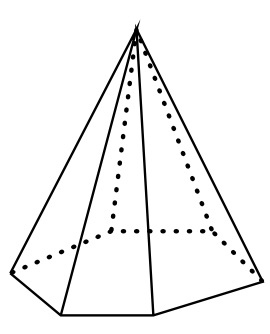
\includegraphics[width=0.3\linewidth]{img/bac_blanc_01.jpg}
  \caption{\label{} Modèle de flacon}
\end{figure}

On donne ci-après une représentation en perspective de cette pyramide notée SA'B'C'D'E'F'.

\begin{figure}[H]
  \centering
  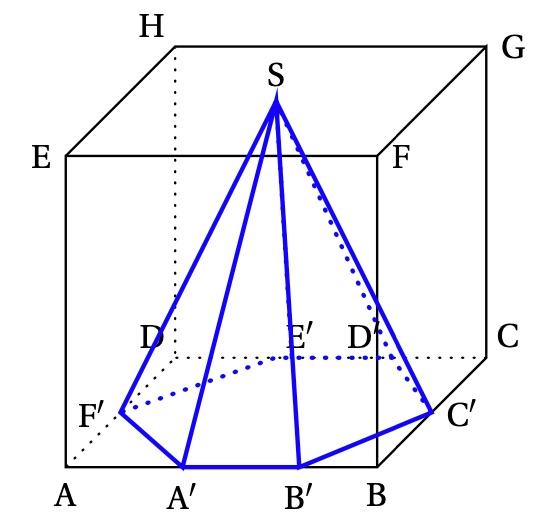
\includegraphics[width=0.6\linewidth]{img/bac_blanc_02.jpg}
  \caption{\label{} Pyramide dans l'espace}
\end{figure}

\begin{itemize}[noitemsep]
  \item La pyramide SA'B'C'D'E'F' est inscrite dans un cube ABCDEFGH d'arête 8 cm.
  \item Le sommet S de la pyramide est le centre de la face EFGH du cube.
  \item La base A'B'C'D'E'F' de cette pyramide est contenue dans la face ABCD du cube.
  \item Les points C'et F'sont les milieux respectifs des segments [BC] et [AD].
  \item Les points A' et B' appartiennent au segment [AB].
  \item Les points D'et E'appartiennent au segment [CD].
  \item Et AA' = A'B' = CD' = E'D' = 3cm.
\end{itemize}

\subsection*{Etude de la pyramide}

On munit l'espace du repère orthonormé $\left(A\mathpunct{} ; \ \vec{\imath}\mathpunct{}, \ \vec{\jmath}\mathpunct{}, \ \vec{k}\right)$ d'origine $A$ et d'unité 1 cm, tel que :

\[
  \vec{\imath} = \frac{1}{8} \overrightarrow{AB} ; 
  \vec{\jmath} = \frac{1}{8} \overrightarrow{AD} ; 
  \vec{k} = \frac{1}{8} \overrightarrow{AE} ;
\]

Ainsi, dans ce repère le point $G$ a pour coordonnées $(8; 8; 8)$ et le point $C$ a pour coordonnées $(8 ; 8 ; 0)$.


\begin{questions}
  \question[1.5] Donner les coordonnées de chacun des points S, A', B', C', E', et F' dans ce repère.
  \question[1] Calculer la longueur du segment [B'C']. La base de la pyramide est-elle un polygone régulier ? (Justifier)
  \question[1] En  utilisant le théorème de Pythagore sur le triangle B'BC' (qui est rectangle en B), vérifier que la longueur de [B'C'] trouvée dans la question 2 est cohérente.
  \question[1.5] Déterminer les coordonées des vecteurs $\overrightarrow{F'E'}$ et $\overrightarrow{B'C'}$. Que peut-on dire de la relation entre ces deux vecteurs ? Que peut-on en déduire des droites $(F'E')$ et $(B'C')$ ?
\end{questions}


\section*{Exercice 2 [6 points] Les suites}

\begin{questions}
  \question[3] Soit la suite $(U_n)$ définie par :
  \[
  \left\{
  \begin{array}{l}
      U_{n+1} = U_n + 3 \\
      U_0 = 2
  \end{array}
  \right.
  \]

  \begin{parts}
    \part[1] Calculer les termes $U_1$, $U_4$, et $U_6$. Il est obligatoire de bien justifier.
    \part[1] Calculer $U_{n+1} - U_n$ pour tout \(n \in \mathbb{N}\) (autrement dit $n$ est entier et $n \geq 0$).
    \part[0.5] La suite est-elle croissante ou décroissante ?
    \part[0.5] D'après le cours sur les suites géométriques et arithmétiques, comment pouvait-on immédiatement - dès la lecture de l'énoncé - dire si la suite allait être croissante ou décroissante ?
\end{parts}

\question[3] Soit la suite $(U_n)$ définie par :
    \[
    \left\{
    \begin{array}{l}
        U_{n+1} = U_n^2 + U_n + 2 \\
        U_0 = 1
    \end{array}
    \right.
    \]

    \begin{parts}
      \part[1] Calculer les termes $U_1$, $U_2$, et $U_3$.
      \part[1] Calculer $U_{n+1} - U_n$ pour tout \(n \in \mathbb{N}\) (autrement dit $n$ est entier et $n \geq 0$).
      \part[1] Connaissant le signe des nombres carrés, que peut-on en déduire sur le signe de $U_{n+1} - U_n$ ? En déduire si la suite est croissante ou décroissante.
  \end{parts}

\end{questions}

\section*{Exercice 3 [9 points] Les fonctions}

\begin{questions}
\question[2] Montrer que la fonction $g(x) = x^2 - 4x - 12$ peut s'écrire sous la forme 
\[
(x-6)(x+2).
\]

\question[0.5] En déduire les solutions de l'équation $g(x)=0$.

\question[0.5] Quelle est l'image de $x=1$ par la fonction $g$ ?

\question[1] Le point $C$ de coordonnées $(1 ; -12)$ appartient-il à la courbe représentative de $g$ ? Qu'en est-il du point $D$ de coordonnées $(-2 ; 0)$ ? Justifier.

\question[2] Construire le tableau de signe de la fonction $g$ sur le domaine de définition $\mathcal{D} = ] - \infty ; + \infty [$.

\question[1] En déduire les solutions de l'inéquation 
\[
g(x) \leq 0.
\]
On prendra le soin de bien écrire les intervalles.

\question[1] L'extremum (maximum ou minimum) d'un polynome de degré 2 du type $a x^2 + bx + c$ est atteint en $x= - \frac{b}{2a}$. Quelles sont les coordonées de l'extremum de la courbe représentative de $g$ ?

\question[1] En vous aidant du signe de $a$ et grâce à la réponse à la question précédente, dresser le tableau de variation de la fonction $g$.

\end{questions}

\section*{Aide}

\begin{itemize}
  \item Un polygone est régulier si et seulement si tous ses côtés ont la même longueur
  \item On peut dire que deux droites sont parallèles si et seulement si leurs vecteurs directeurs (les vecteurs qui suivent la direction de la droite) sont colinéaires.
  \item On dit que 2 vecteurs $\overrightarrow{AB}$ et $\overrightarrow{CD}$ respectivement de coordonées $x_{AB}, y_{AB}, z_{AB}$ et $x_{CD}, y_{CD}, z_{CD}$ sont colinéires si et seulement si on peut écrire 
  \[
  \overrightarrow{AB} = \alpha \cdot \overrightarrow{CD}
  \]
 c'est-à-dire
  \[
  \begin{pmatrix}
    x_{AB} \\
    y_{AB} \\ 
    z_{AB}
  \end{pmatrix}
  = 
  \alpha \cdot
  \begin{pmatrix}
    x_{CD} \\
    y_{CD} \\ 
    z_{CD}
  \end{pmatrix}
\] 
autrement dit 
\[
  \begin{pmatrix}
    x_{AB} \\
    y_{AB} \\ 
    z_{AB}
  \end{pmatrix}
  =
  \begin{pmatrix}
    \alpha \cdot x_{CD} \\
    \alpha \cdot y_{CD} \\ 
    \alpha \cdot z_{CD}
  \end{pmatrix}
\] 
\end{itemize}


\end{document}
